% Figure from MATH 591 notes, section 59. Compile with the notes preamble.
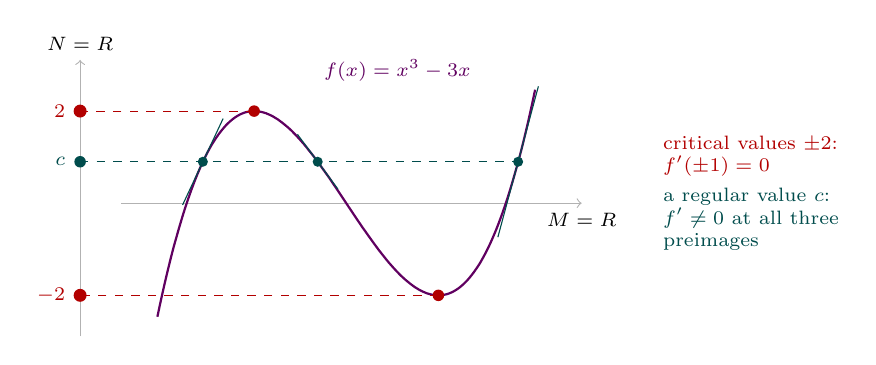
\begin{tikzpicture}[scale=1.3]
\draw[->, gray!60] (-2.2,0) -- (2.3,0) node[below, font=\scriptsize, text=black] {$M = \mathbb{R}$};
\draw[->, gray!60] (-2.6,-1.3) -- (-2.6,1.4) node[above, font=\scriptsize, text=black] {$N = \mathbb{R}$};
\draw[violet!75!black, thick] plot[smooth] coordinates {(-1.845,-1.109) (-1.822,-1.000) (-1.799,-0.895) (-1.776,-0.793) (-1.753,-0.695) (-1.730,-0.600) (-1.707,-0.508) (-1.684,-0.420) (-1.660,-0.335) (-1.637,-0.254) (-1.614,-0.176) (-1.591,-0.100) (-1.568,-0.028) (-1.545,0.040) (-1.522,0.106) (-1.499,0.169) (-1.476,0.229) (-1.453,0.286) (-1.430,0.340) (-1.407,0.392) (-1.384,0.440) (-1.361,0.486) (-1.338,0.529) (-1.315,0.570) (-1.291,0.608) (-1.268,0.643) (-1.245,0.676) (-1.222,0.706) (-1.199,0.734) (-1.176,0.760) (-1.153,0.783) (-1.130,0.804) (-1.107,0.823) (-1.084,0.840) (-1.061,0.854) (-1.038,0.867) (-1.015,0.877) (-0.992,0.886) (-0.969,0.892) (-0.946,0.896) (-0.922,0.899) (-0.899,0.900) (-0.876,0.899) (-0.853,0.896) (-0.830,0.892) (-0.807,0.886) (-0.784,0.879) (-0.761,0.869) (-0.738,0.859) (-0.715,0.847) (-0.692,0.833) (-0.669,0.819) (-0.646,0.802) (-0.623,0.785) (-0.600,0.766) (-0.577,0.747) (-0.553,0.726) (-0.530,0.704) (-0.507,0.680) (-0.484,0.656) (-0.461,0.631) (-0.438,0.605) (-0.415,0.579) (-0.392,0.551) (-0.369,0.522) (-0.346,0.493) (-0.323,0.464) (-0.300,0.433) (-0.277,0.402) (-0.254,0.370) (-0.231,0.338) (-0.208,0.306) (-0.184,0.273) (-0.161,0.240) (-0.138,0.206) (-0.115,0.172) (-0.092,0.138) (-0.069,0.104) (-0.046,0.069) (-0.023,0.035) (0.000,0.000) (0.023,-0.035) (0.046,-0.069) (0.069,-0.104) (0.092,-0.138) (0.115,-0.172) (0.138,-0.206) (0.161,-0.240) (0.185,-0.273) (0.208,-0.306) (0.231,-0.338) (0.254,-0.370) (0.277,-0.402) (0.300,-0.433) (0.323,-0.464) (0.346,-0.493) (0.369,-0.522) (0.392,-0.551) (0.415,-0.579) (0.438,-0.605) (0.461,-0.631) (0.484,-0.656) (0.507,-0.680) (0.530,-0.704) (0.554,-0.726) (0.577,-0.747) (0.600,-0.766) (0.623,-0.785) (0.646,-0.802) (0.669,-0.819) (0.692,-0.833) (0.715,-0.847) (0.738,-0.859) (0.761,-0.869) (0.784,-0.879) (0.807,-0.886) (0.830,-0.892) (0.853,-0.896) (0.876,-0.899) (0.899,-0.900) (0.922,-0.899) (0.946,-0.896) (0.969,-0.892) (0.992,-0.886) (1.015,-0.877) (1.038,-0.867) (1.061,-0.854) (1.084,-0.840) (1.107,-0.823) (1.130,-0.804) (1.153,-0.783) (1.176,-0.760) (1.199,-0.734) (1.222,-0.706) (1.245,-0.676) (1.268,-0.643) (1.292,-0.608) (1.315,-0.570) (1.338,-0.529) (1.361,-0.486) (1.384,-0.440) (1.407,-0.392) (1.430,-0.340) (1.453,-0.286) (1.476,-0.229) (1.499,-0.169) (1.522,-0.106) (1.545,-0.040) (1.568,0.028) (1.591,0.100) (1.614,0.176) (1.637,0.254) (1.660,0.335) (1.684,0.420) (1.707,0.508) (1.730,0.600) (1.753,0.695) (1.776,0.793) (1.799,0.895) (1.822,1.000) (1.845,1.109)};
\draw[red!70!black, dashed] (-0.900,0.900) -- (-2.6,0.900);
\fill[red!70!black] (-0.900,0.900) circle (1.6pt);
\fill[red!70!black] (-2.6,0.900) circle (1.8pt);
\draw[red!70!black, dashed] (0.900,-0.900) -- (-2.6,-0.900);
\fill[red!70!black] (0.900,-0.900) circle (1.6pt);
\fill[red!70!black] (-2.6,-0.900) circle (1.8pt);
\node[red!70!black, font=\scriptsize, anchor=east] at (-2.65,0.900) {$2$};
\node[red!70!black, font=\scriptsize, anchor=east] at (-2.65,-0.900) {$-2$};
\draw[teal!60!black, dashed] (-2.6,0.405) -- (1.679,0.405);
\fill[teal!60!black] (-2.6,0.405) circle (1.6pt);
\node[teal!60!black, font=\scriptsize, anchor=east] at (-2.65,0.405) {$c$};
\fill[teal!60!black] (-1.401,0.405) circle (1.4pt);
\draw[teal!60!black] (-1.599,-0.017) -- (-1.203,0.827);
\fill[teal!60!black] (-0.279,0.405) circle (1.4pt);
\draw[teal!60!black] (-0.477,0.673) -- (-0.081,0.137);
\fill[teal!60!black] (1.679,0.405) circle (1.4pt);
\draw[teal!60!black] (1.481,-0.332) -- (1.877,1.142);
\node[font=\scriptsize, violet!75!black] at (0.5,1.3) {$f(x) = x^3 - 3x$};
\node[font=\scriptsize, align=left, anchor=west] at (3.0,0.1) {\textcolor{red!70!black}{critical values $\pm 2$:}\\ \textcolor{red!70!black}{$f'(\pm 1) = 0$}\\[3pt] \textcolor{teal!60!black}{a regular value $c$:}\\ \textcolor{teal!60!black}{$f' \ne 0$ at all three}\\ \textcolor{teal!60!black}{preimages}};
\end{tikzpicture}
